\chapter{\altGerEng{Anhang}{Appendix}}


\section{Thonny}\label{appendix:A1}
Thonny is an integrated development environment (IDE) for MicroPython, which makes it easier for users to program, primarily when used with Raspberry Pi Pico. The Raspberry Pi Pico can be conveniently programmed with MicroPython firmware. Thonny also provides the users with an environment that allows them to perform multiple operations on the board’s ports, such as GPIO, sensors, and actuators. For these reasons, Thonny, combined with microPython for Raspberry Pi Pico, makes it entirely possible to learn about embedded systems and even build real-world applications without coming to terms with the usual synthetic low-level languages used in actual embedded systems.

\section{STM32CubeIDE}\label{appendix:A2}

STM32CubeIDE is a development environment specifically designed for STM32 microcontrollers. It combines several tools into a single platform, including a code editor, debugger, and a graphical interface for configuring microcontroller settings. One of its best features is STM32CubeMX, which allows users to set up pin assignments and peripherals through a visual interface, simplifying the initial setup process. Developers can write, compile, and debug their code in one place. STM32CubeIDE is compatible with Windows, Linux, and macOS, making it easier to work with STM32 development boards.

\section{Output vs original at different baud rates}\label{appendix:A3}


\begin{figure}[t]
    \centering
    
    % First row of subfigures
    \begin{subfigure}[t]{0.48\textwidth}
        \centering
        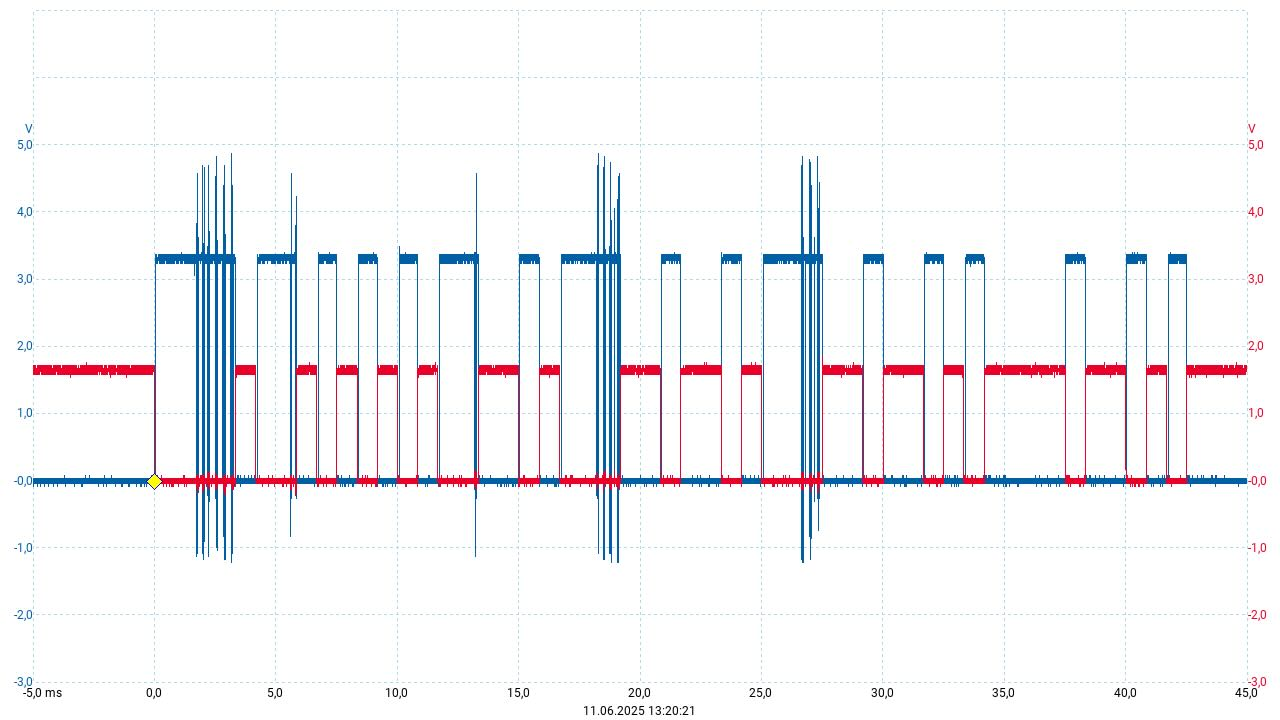
\includegraphics[width=1\textwidth]{fig/compvs/comp vs original 5cm 1200 br.jpg}
        \caption{Baud rate 1200}
        \label{fig:A.1-a}
    \end{subfigure}
    \hfill
    \begin{subfigure}[t]{0.48\textwidth}
        \centering
        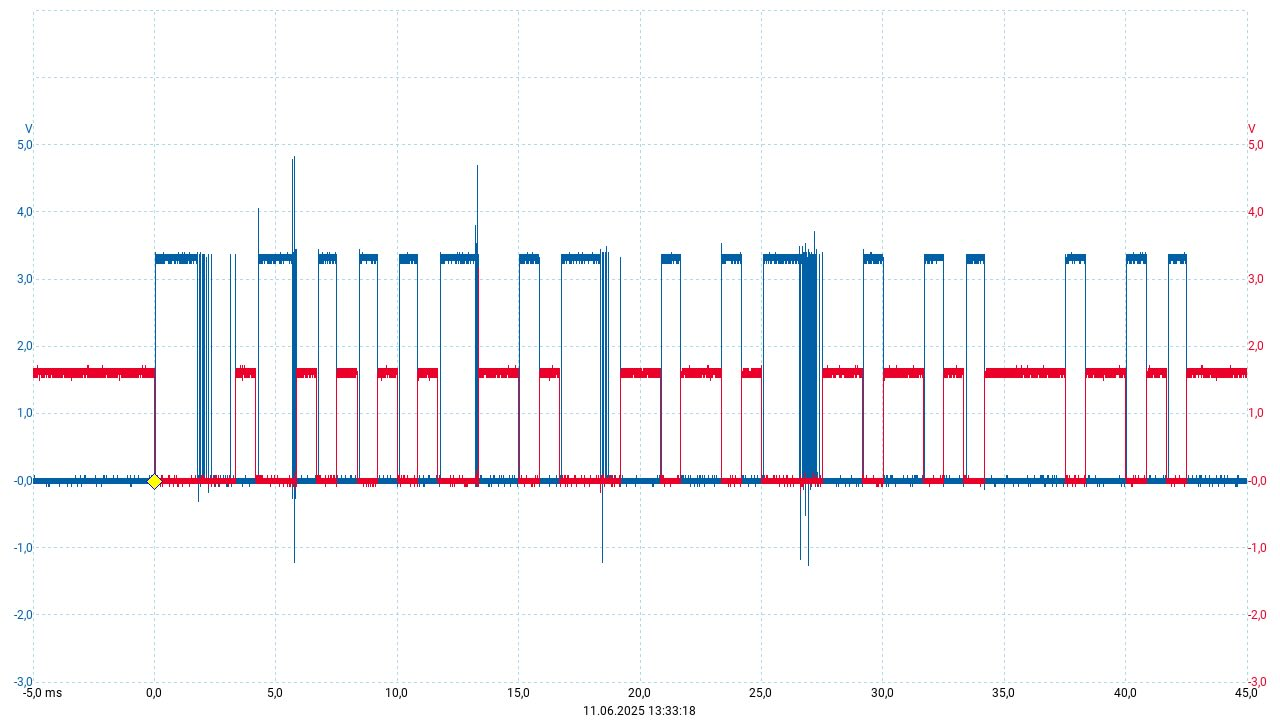
\includegraphics[width=1\textwidth]{fig/compvs/comp vs original 5cm 2400 br.jpg}
        \caption{Baud rate 2400}
        \label{fig:A.1-b}
    \end{subfigure}
    
    \vspace{0.5em} % Small vertical space between rows

    % Second row of subfigures
    \begin{subfigure}[t]{0.48\textwidth}
        \centering
        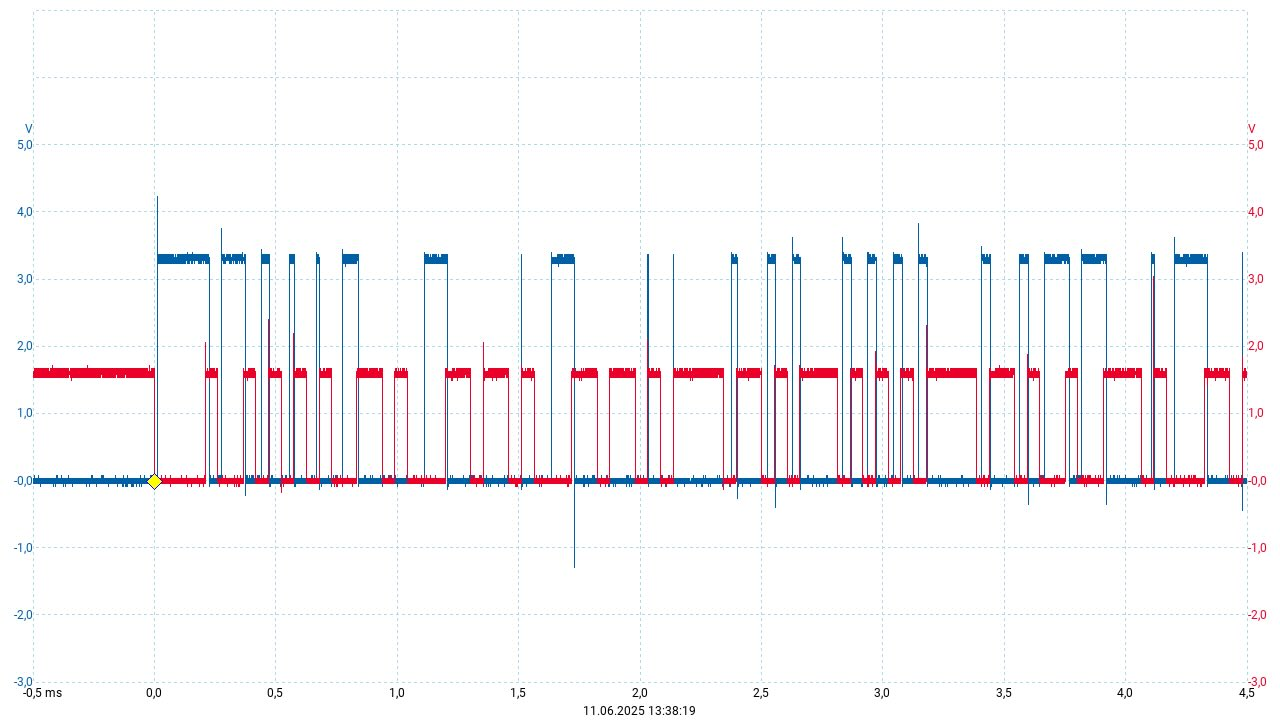
\includegraphics[width=1\textwidth]{fig/compvs/comp vs original 5cm 19200 br.jpg}
        \caption{Baud rate 19200}
        \label{fig:A.1-c}
    \end{subfigure}
    \hfill
    \begin{subfigure}[t]{0.48\textwidth}
        \centering
        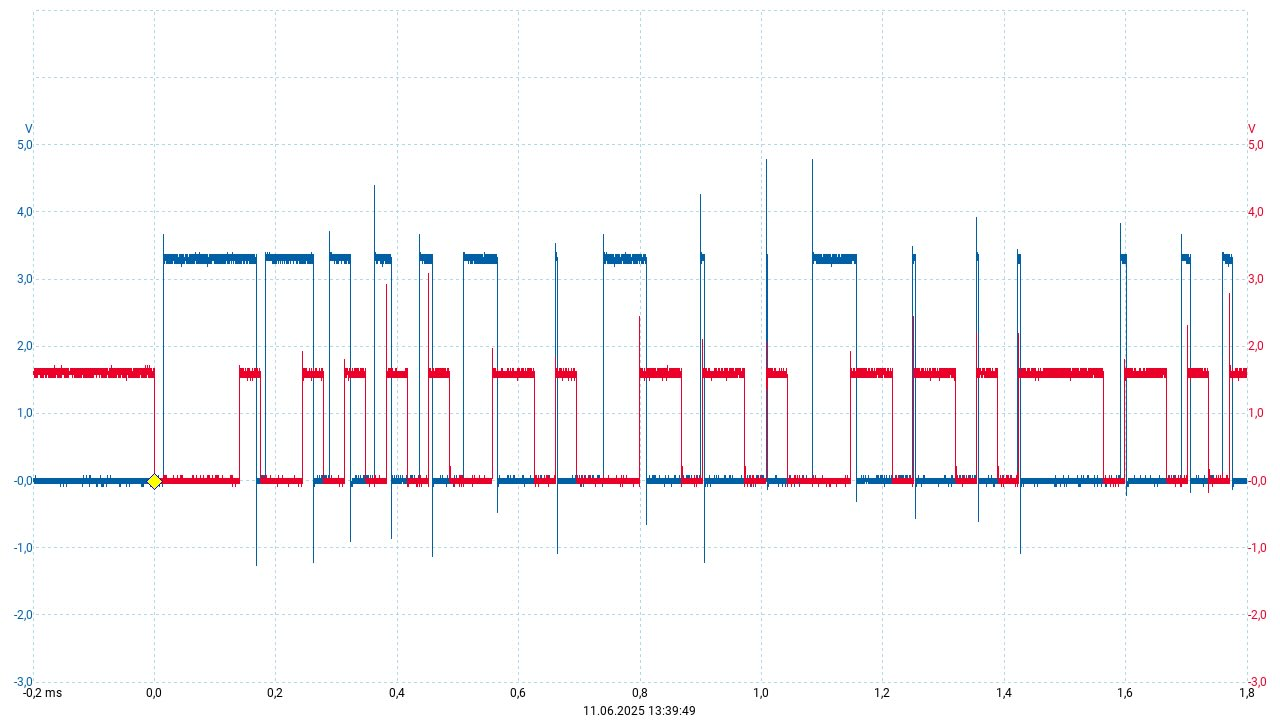
\includegraphics[width=1\textwidth]{fig/compvs/comp vs original 5cm 28800 br.jpg}
        \caption{Baud rate 28800}
        \label{fig:A.1-d}
    \end{subfigure}

    \caption{output vs original at different baud rates at 5cm.}
    \label{fig:A.1}
\end{figure}


\begin{figure}[t]
    \centering
    
    % First row of subfigures
    \begin{subfigure}[t]{0.48\textwidth}
        \centering
        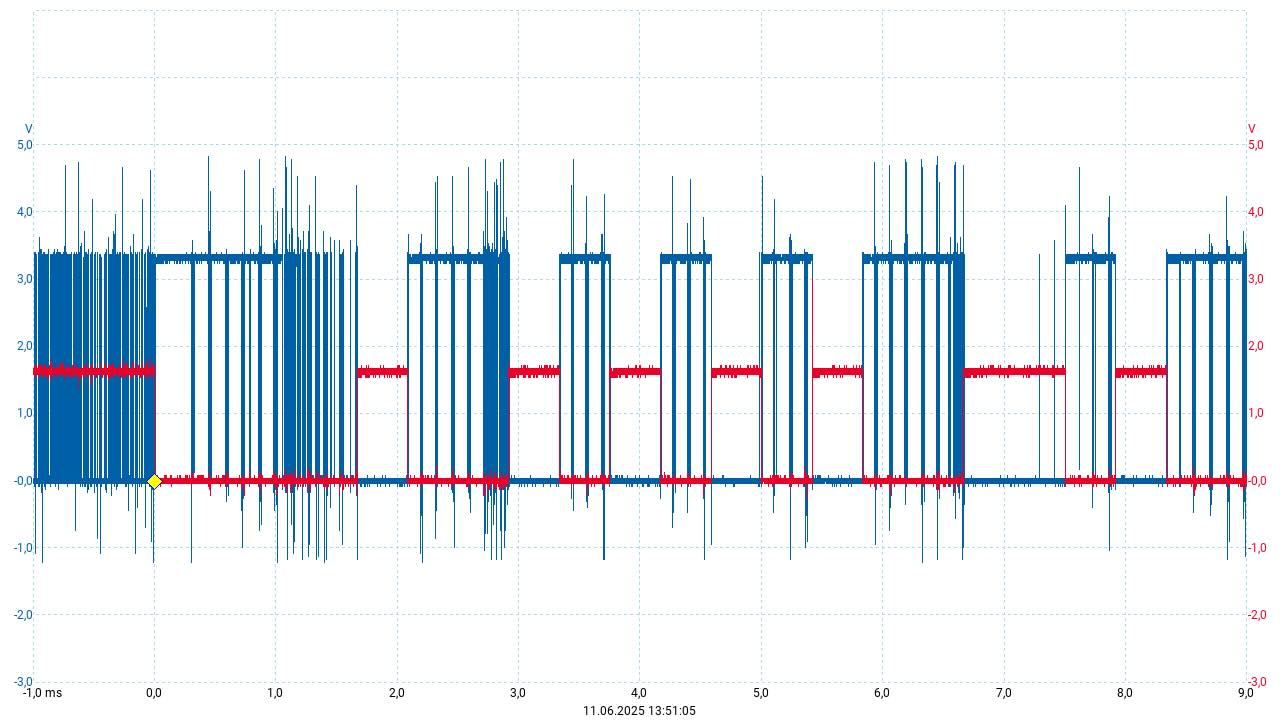
\includegraphics[width=1\textwidth]{fig/compvs/comp vs original 15cm 2400.jpg}
        \caption{Baud rate 1200}
        \label{fig:A.3-a}
    \end{subfigure}
    \hfill
    \begin{subfigure}[t]{0.48\textwidth}
        \centering
        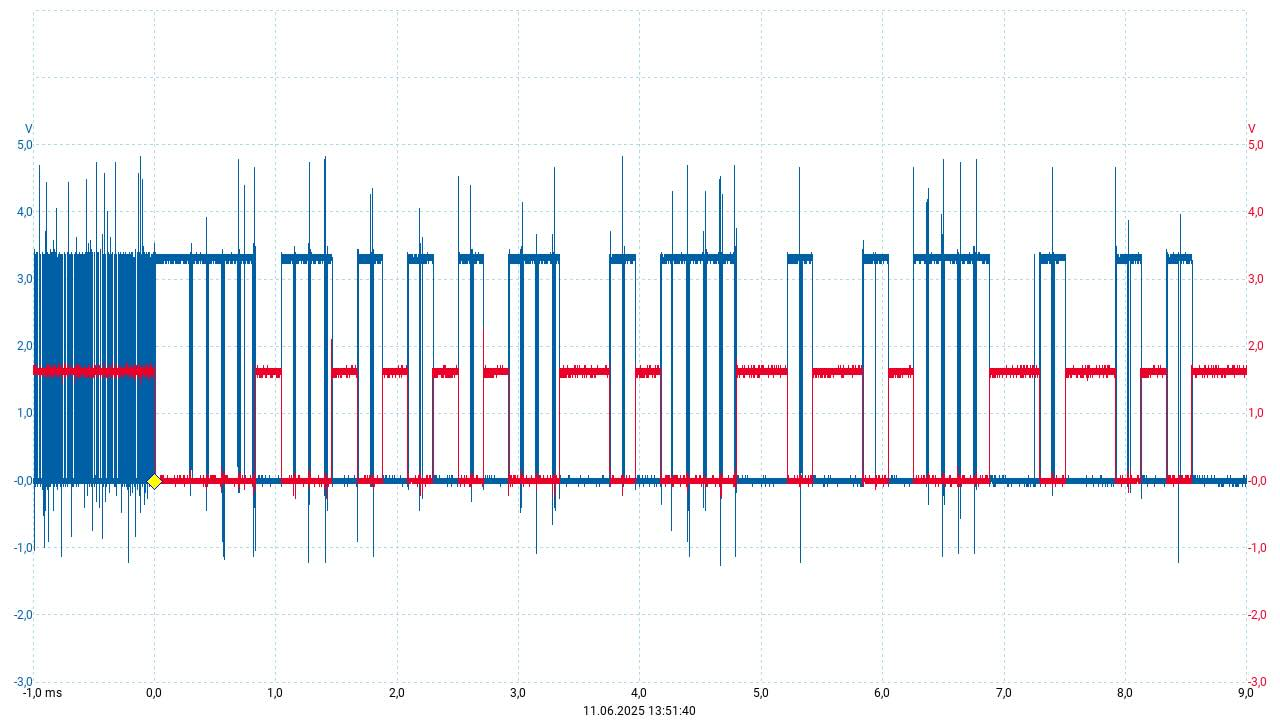
\includegraphics[width=1\textwidth]{fig/compvs/comp vs original 15cm 4800.jpg}
        \caption{Baud rate 2400}
        \label{fig:A.3-b}
    \end{subfigure}
    
    \vspace{0.5em} % Small vertical space between rows

    % Second row of subfigures
    \begin{subfigure}[t]{0.48\textwidth}
        \centering
        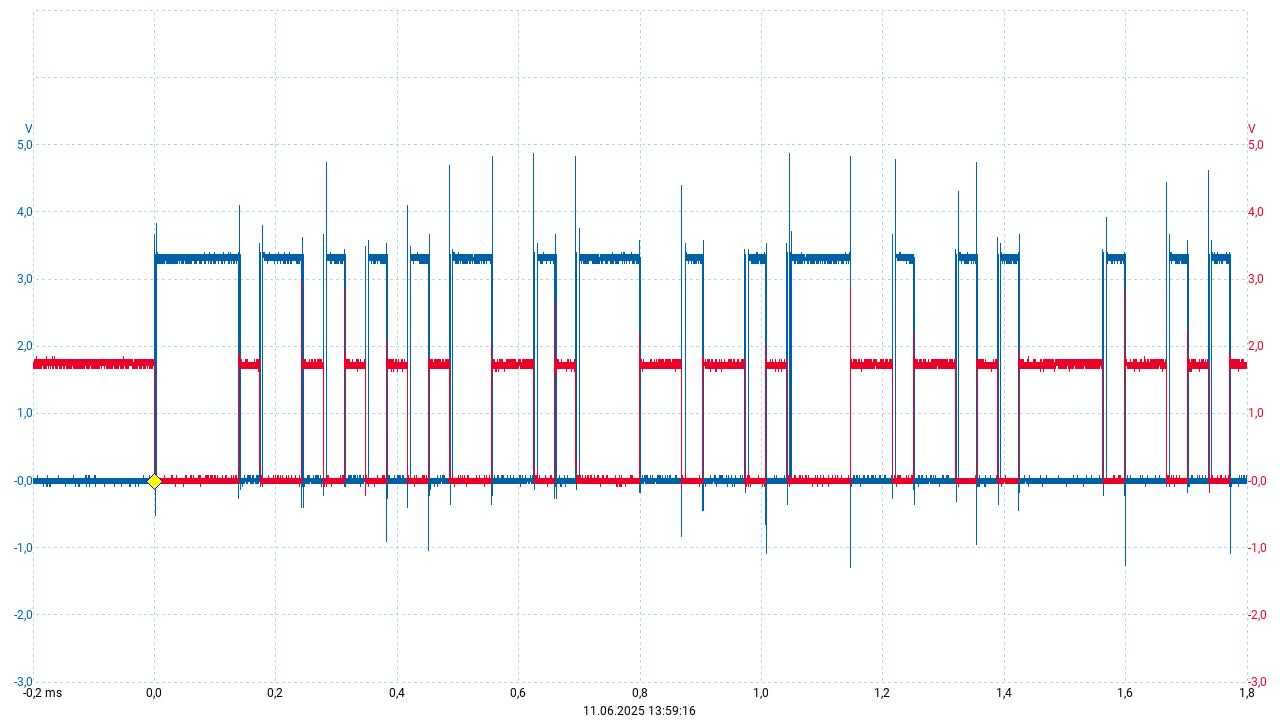
\includegraphics[width=1\textwidth]{fig/compvs/comp vs original 15cm 28800.jpg}
        \caption{Baud rate 28800}
        \label{fig:A.3-c}
    \end{subfigure}
    \hfill

    \caption{output vs original at different baud rates at 15cm.}
    \label{fig:A.3}
\end{figure}








